\chapter{Especificação de requisitos do trabalho}

\label{CAP4}


% definir técnicas, processos e sistemas, procedimentos que vão compor o sistema

Neste capítulo serão descritas as necessidades básicas levantadas para que o projeto funcione como esperado.

Na figura \ref{fig:class_diagram} pode ser visto o diagrama de classes que define o sistema como um todo.

\begin{figure}[hp]
    \centering
    
    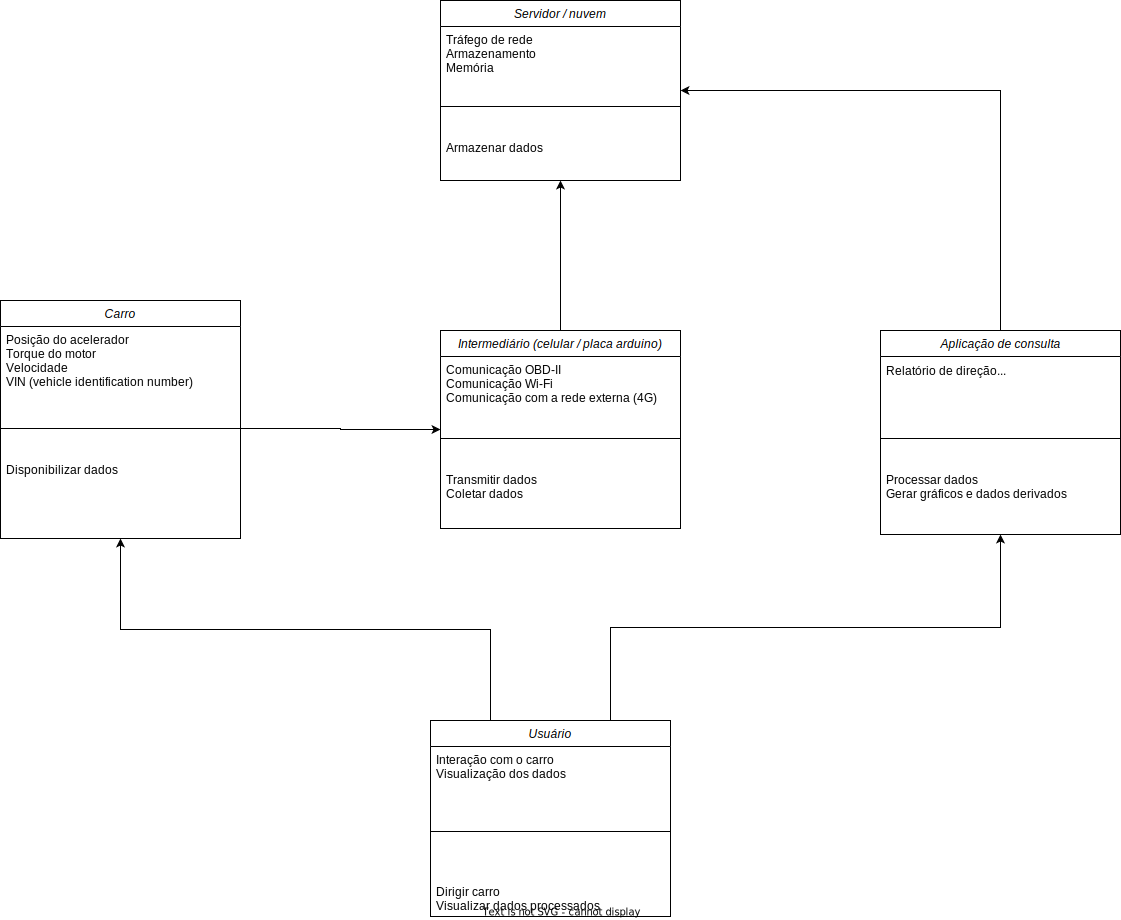
\includegraphics[scale=0.4]{figures/coleta_dados_carro}
    
    \caption{Diagrama de classes com visão mais abstrata do sistema}
    
    \label{fig:class_diagram}
\end{figure}

\section{Requisitos funcionais}
\begin{itemize}
    \item \textbf{Conexão OBD-II:} o aplicativo se comunica com a interface do carro, requisitando apenas as informações definidas, durante o projeto, como relevantes.
    
    \item \textbf{Conexão do celular à \textit{internet}:} transmissão de dados coletados para a nuvem.
    
    \item \textbf{Plataforma de recepção na nuvem:} armazenamento dos dados coletados todos na plataforma de \textit{cloud} definida.
    
    \item \textbf{Histórico de Rotas:} capacidade de armazenar e acessar informações detalhadas sobre os trajetos percorridos por um veículo ao longo do tempo; este recurso é crucial para oferecer aos usuários e administradores uma visão retrospectiva das atividades de um veículo, permitindo uma compreensão abrangente dos padrões de movimentação e comportamento de condução.
\end{itemize}

\section{Requisitos não-funcionais}

\begin{itemize}
    \item \textbf{Conexão contínua com a \textit{internet}:} conexão não para por muito tempo, análise contínua dos dados coletados.
    
    % , além de gerar desconfiança por parte do usuário, ao perceber que não há consistência no sistema.
    
    \item \textbf{Interface sem reconexão manual com a \textit{internet} e \textit{bluetooth}:} re-estabelecimento da conexão com o OBD e a \textit{internet} sem interferência do usuário assim que for ligada novamente; em outras palavras, um sistema \textit{plug and play}.
    
    \item \textbf{Informações relevantes e corretas:} dados apresentados no relatório de direção com nexo para o usuário; apenas meta-informações chegam ao usuário final, passando por "filtro de plausibilidade".
    
    % , para que, mais uma vez, a confiança de quem usará o sistema não seja perdida ao deparar-se com valores \textit{outliers} nas análises geradas.
    
    \item \textbf{Memória e armazenamento em nuvem suficientes:} espaço máximo em nuvem que pode ser usado claramente sinalizado para o usuário ao usar o sistema; além de sinalização de que suas informações não serão mais coletadas assim que o armazenamento seja ocupado por completo.
    
    \item \textbf{Segurança de dados:} pessoas não-autorizadas não podem ter acesso aos dados coletados no veículo de cada usuário.
\end{itemize}

% \subsection{}
% \subsection{}
% \subsection{}


